\KOMAoptions{paper=A3}
\recalctypearea
\section{Fractal Fun}
\begin{topics}
Everthing but not actually everything if you think hard enough :)
\end{topics}
\subsection{L-Systems}{\label{pp:lsystems}}
Lindenmayer system, shortly L-system is a recursive system to generate self-similar patterns.
Simply put, it contains variables, constants, an axiom and rules.

In fact, we have already seen its example \hyperref[pp:thuemorsesequence]{here}. So, let's take that as a reference. We can generate the Thue-Morse Sequence using the below L-System
\begin{description}
	\item[variables] 0,1
	\item[constants] none
	\item[axiom] 0 (start with 0)
	\item[rules] 0 $\rightarrow$ 01, 1 $\rightarrow$ 10 (replace 0 by 01 in next step and 1 by 10)
\end{description}
This produces the following sequences
\begin{description}
	\item[Iterate 0] 0
	\item[Iterate 1] 01
	\item[Iterate 2] 0110
	\item[Iterate 3] 01101001
	\item[Iterate 4] 0110100110010110 and so on
\end{description}
\subsubsection{Dragon Curve}{\label{pp:dragoncurve}}
\begin{description}
	\item[variables] F,G
	\item[constants] +--
	\item[axiom] F
	\item[rules] F $\rightarrow$ F+G, G $\rightarrow$ F--G
\end{description}
The generated sequence is F+G+F--G+F+G--F--G+F+G+F--G--F+G--F--G$\ldots$. Consider F, G as moving forward and + (--) as turning left (right) by 90$^\circ$.

\textbf{Problem Statement:}\\
Draw the corresponding curve using \verb!turtleSim! with appropriate scaling such that it roughly takes same width and height for all iterates.
\begin{tcolorbox}[breakable, enhanced, sharpish corners]%, colback = white]
	\href{https://github.com/paramrathour/CS-101/tree/main/Starter Codes/Dragon Curve.cpp}{\textbf{Starter Code}}
\end{tcolorbox}
\begin{figure}[H]
	\centering
	\begin{subfigure}{0.1\linewidth}
		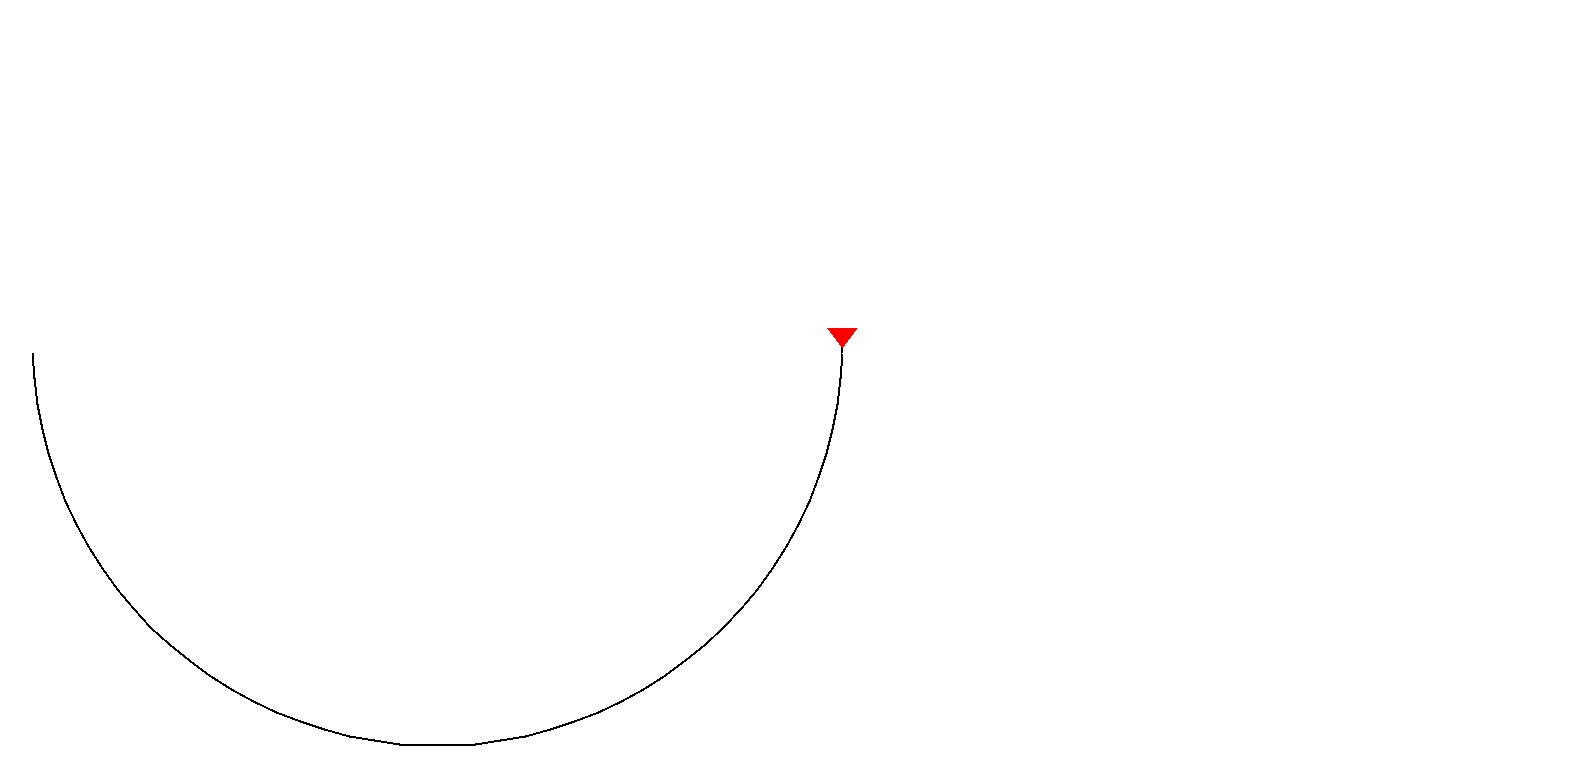
\includegraphics[width = \linewidth]{Dragon Curve/1.png}
		\caption{Iterate 1}
	\end{subfigure}
	\begin{subfigure}{0.08\linewidth}
		\includegraphics[width = \linewidth]{Dragon Curve/2.png}
		\caption{Iterate 2}
	\end{subfigure}
	\begin{subfigure}{0.12\linewidth}
		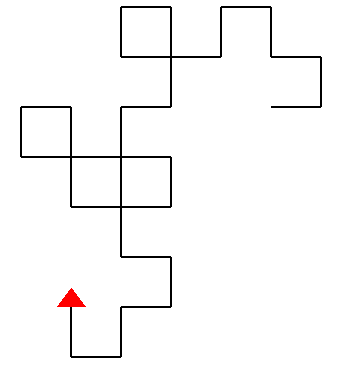
\includegraphics[width = \linewidth]{Dragon Curve/5.png}
		\caption{Iterate 5}
	\end{subfigure}
	\begin{subfigure}{0.16\linewidth}
		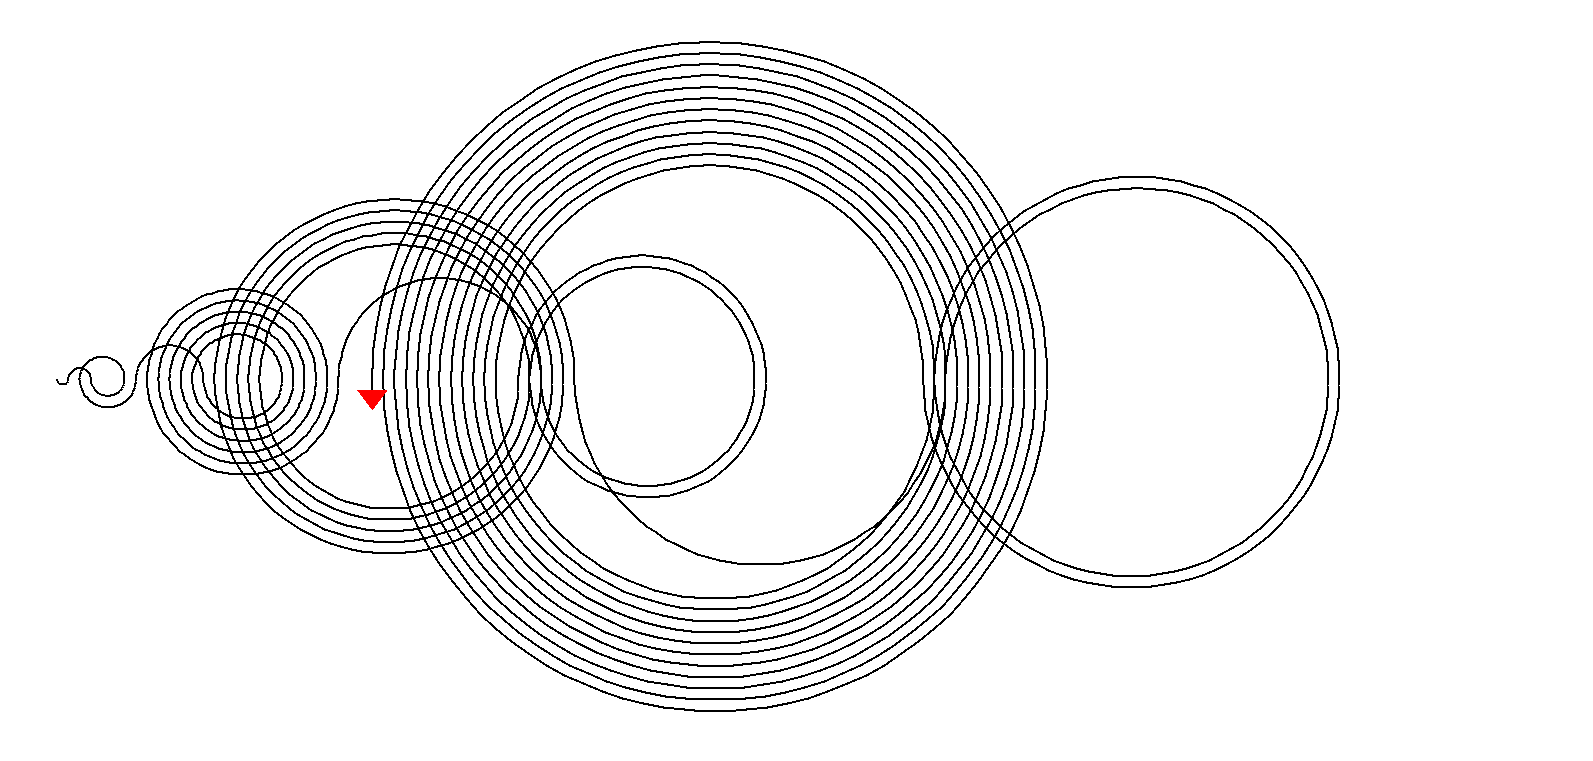
\includegraphics[width = \linewidth]{Dragon Curve/7.png}
		\caption{Iterate 7}
	\end{subfigure}
	\begin{subfigure}{0.09\linewidth}
		\includegraphics[width = \linewidth]{Dragon Curve/10.png}
		\caption{Iterate 10}
	\end{subfigure}
	\begin{subfigure}{0.18\linewidth}
		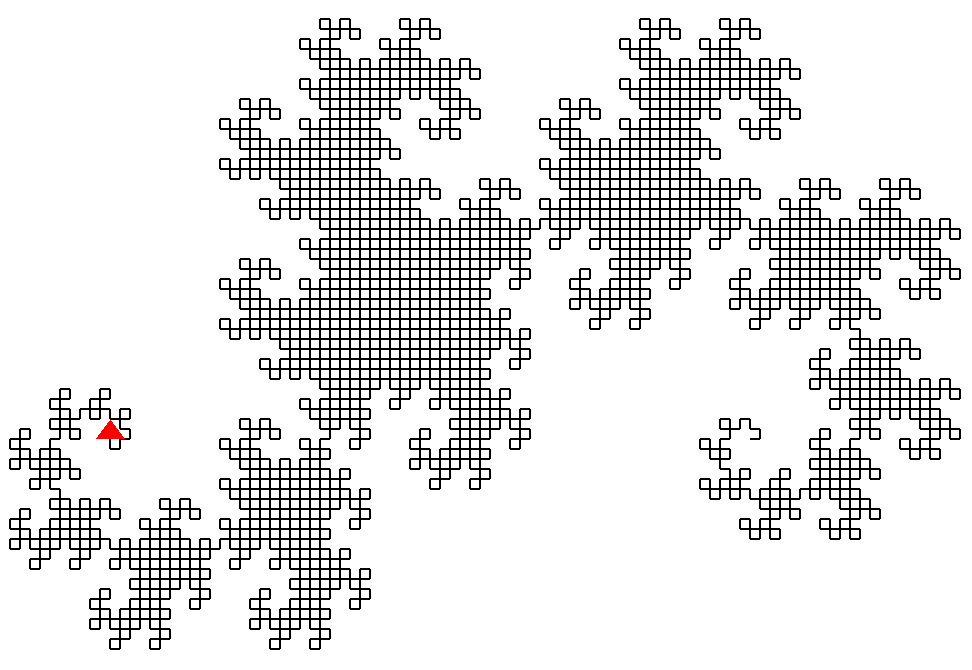
\includegraphics[width = \linewidth]{Dragon Curve/12.png}
		\caption{Iterate 12}
	\end{subfigure}
	\begin{subfigure}{0.18\linewidth}
		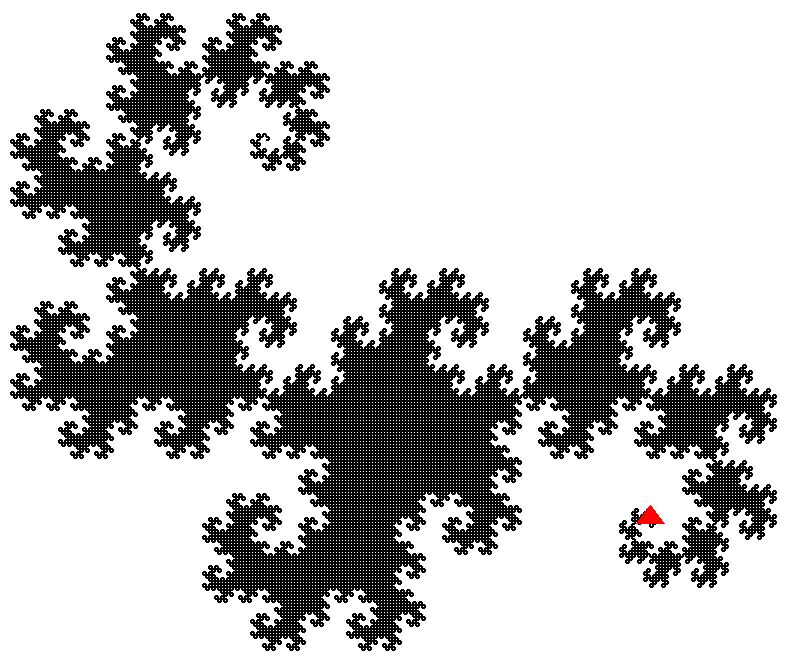
\includegraphics[width = \linewidth]{Dragon Curve/15.png}
		\caption{Iterate 15}
	\end{subfigure}
	\caption{Dragon Curve iterates}
\end{figure}
\vspace{-2em}
\subsubsection{Sierpi\'nski Arrowhead Curve}{\label{pp:sierpinskicurve}}
\begin{description}
	\item[variables] A,B
	\item[constants] +--
	\item[axiom] A
	\item[rules] A $\rightarrow$ B--A--B, B $\rightarrow$ A+B+A
\end{description}
Try generating this. Here, A, B denote moving forward and + (--) denote turning left (right) by 60$^\circ$.

\textbf{Problem Statement:}\\
Again, draw the corresponding curve using \verb!turtleSim! with appropriate scaling such that it roughly takes same width and height for all iterates.
\begin{tcolorbox}[breakable, enhanced, sharpish corners]%, colback = white]
	\href{https://github.com/paramrathour/CS-101/tree/main/Starter Codes/Sierpi\'nski Arrowhead Curve.cpp}{\textbf{Starter Code}}
\end{tcolorbox}
\begin{figure}[H]
	\centering
	\begin{subfigure}{0.18\linewidth}
		\includegraphics[width = \linewidth]{Sierpiński Arrowhead Curve/2.png}
		\caption{Iterate 2}
	\end{subfigure}
	\begin{subfigure}{0.18\linewidth}
		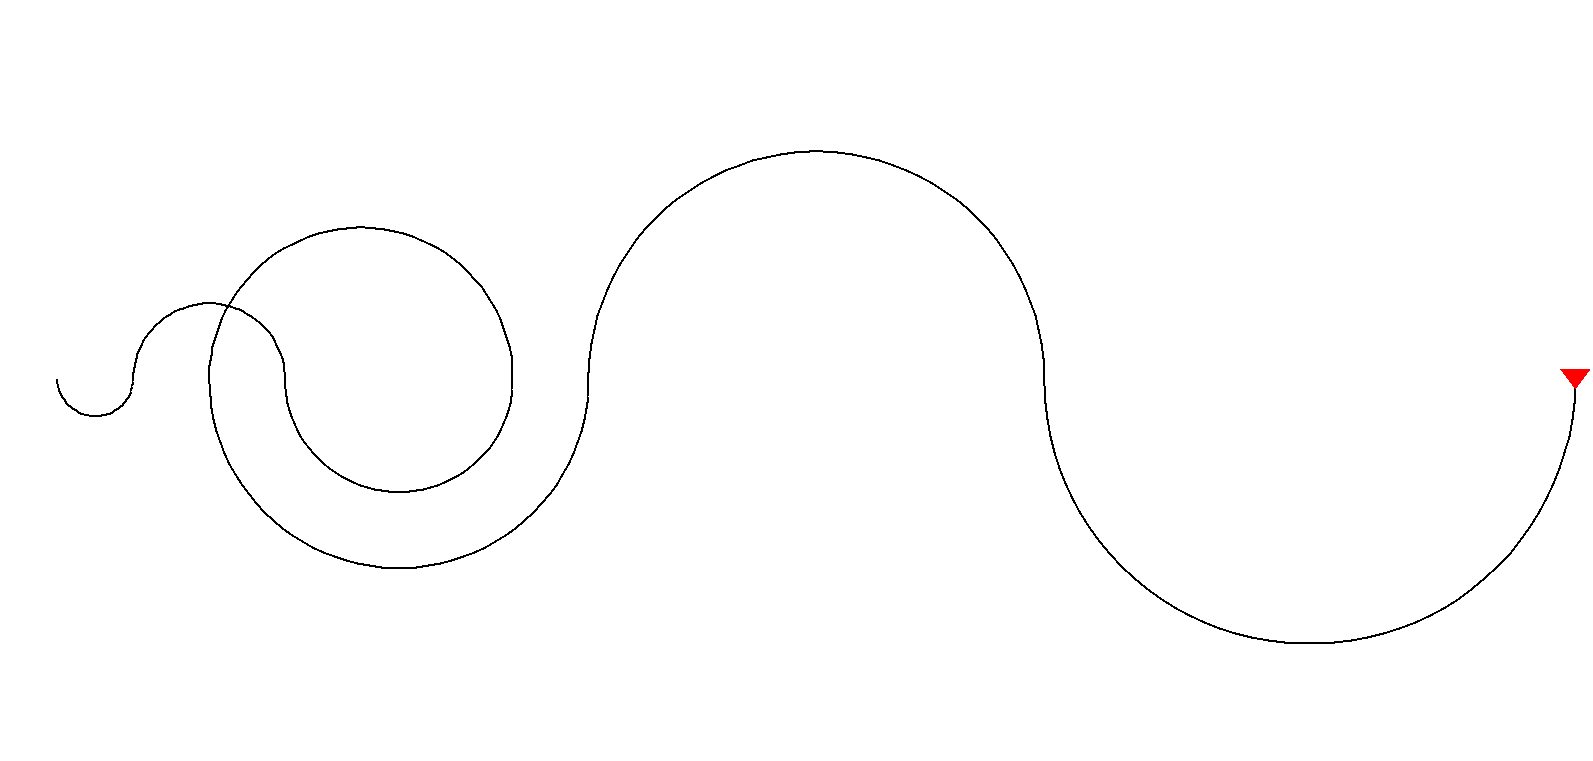
\includegraphics[width = \linewidth]{Sierpiński Arrowhead Curve/4.png}
		\caption{Iterate 4}
	\end{subfigure}
	\begin{subfigure}{0.18\linewidth}
		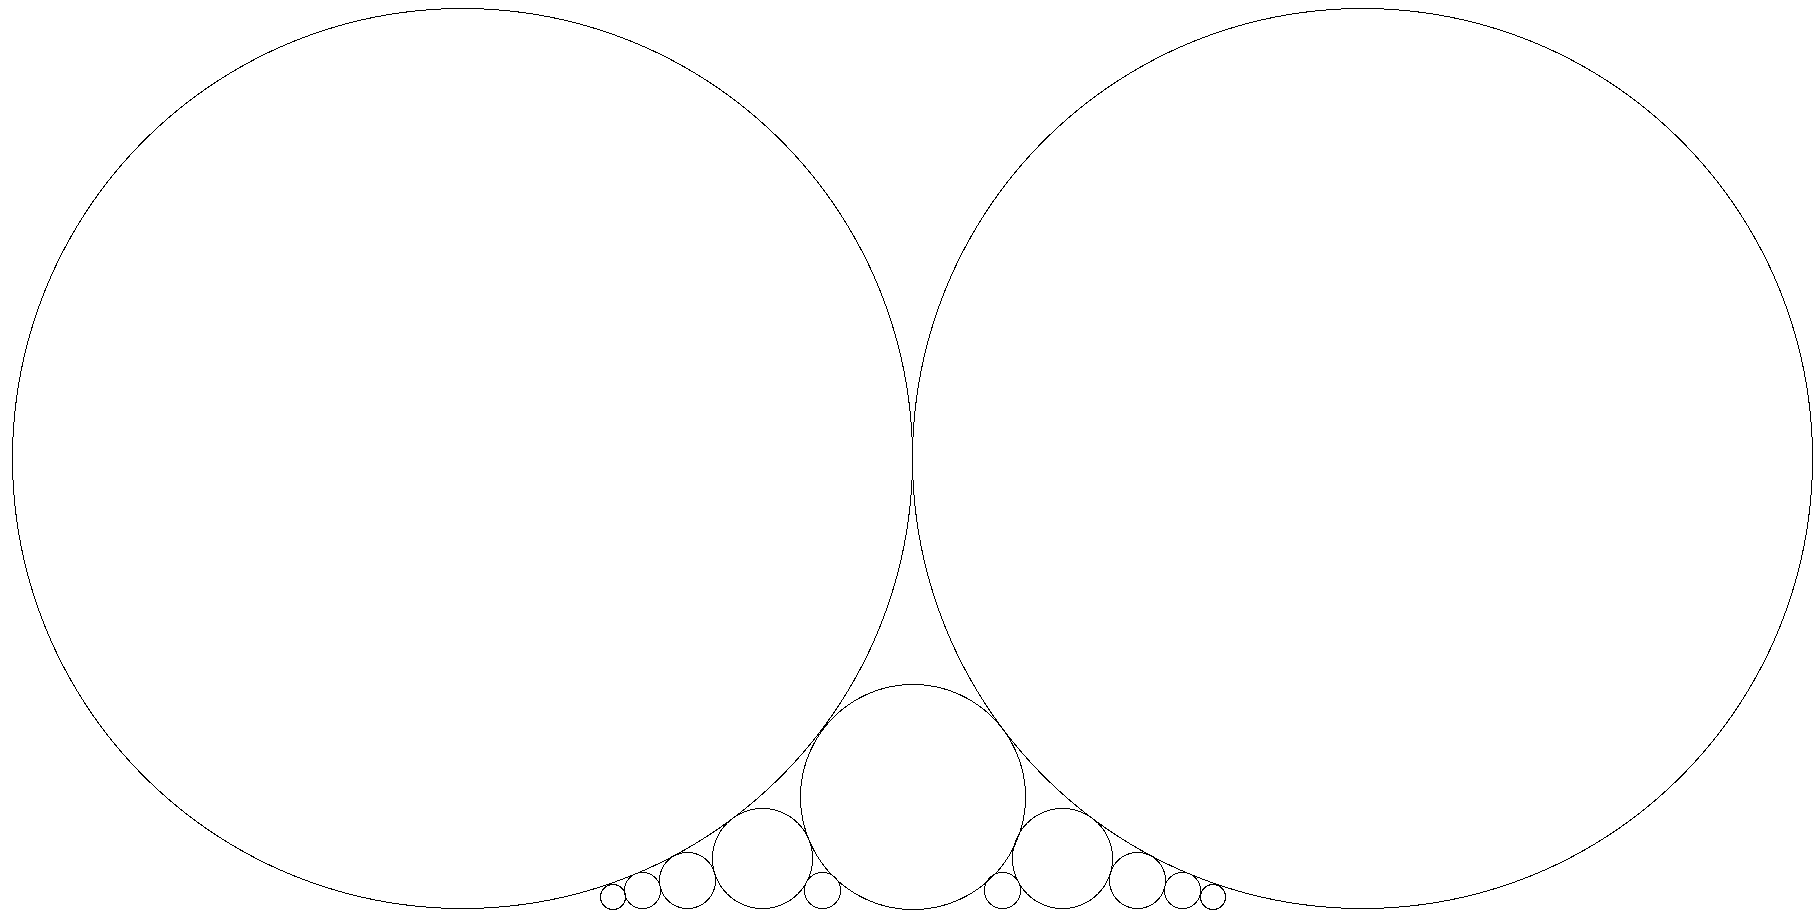
\includegraphics[width = \linewidth]{Sierpiński Arrowhead Curve/6.png}
		\caption{Iterate 6}
	\end{subfigure}
	\begin{subfigure}{0.18\linewidth}
		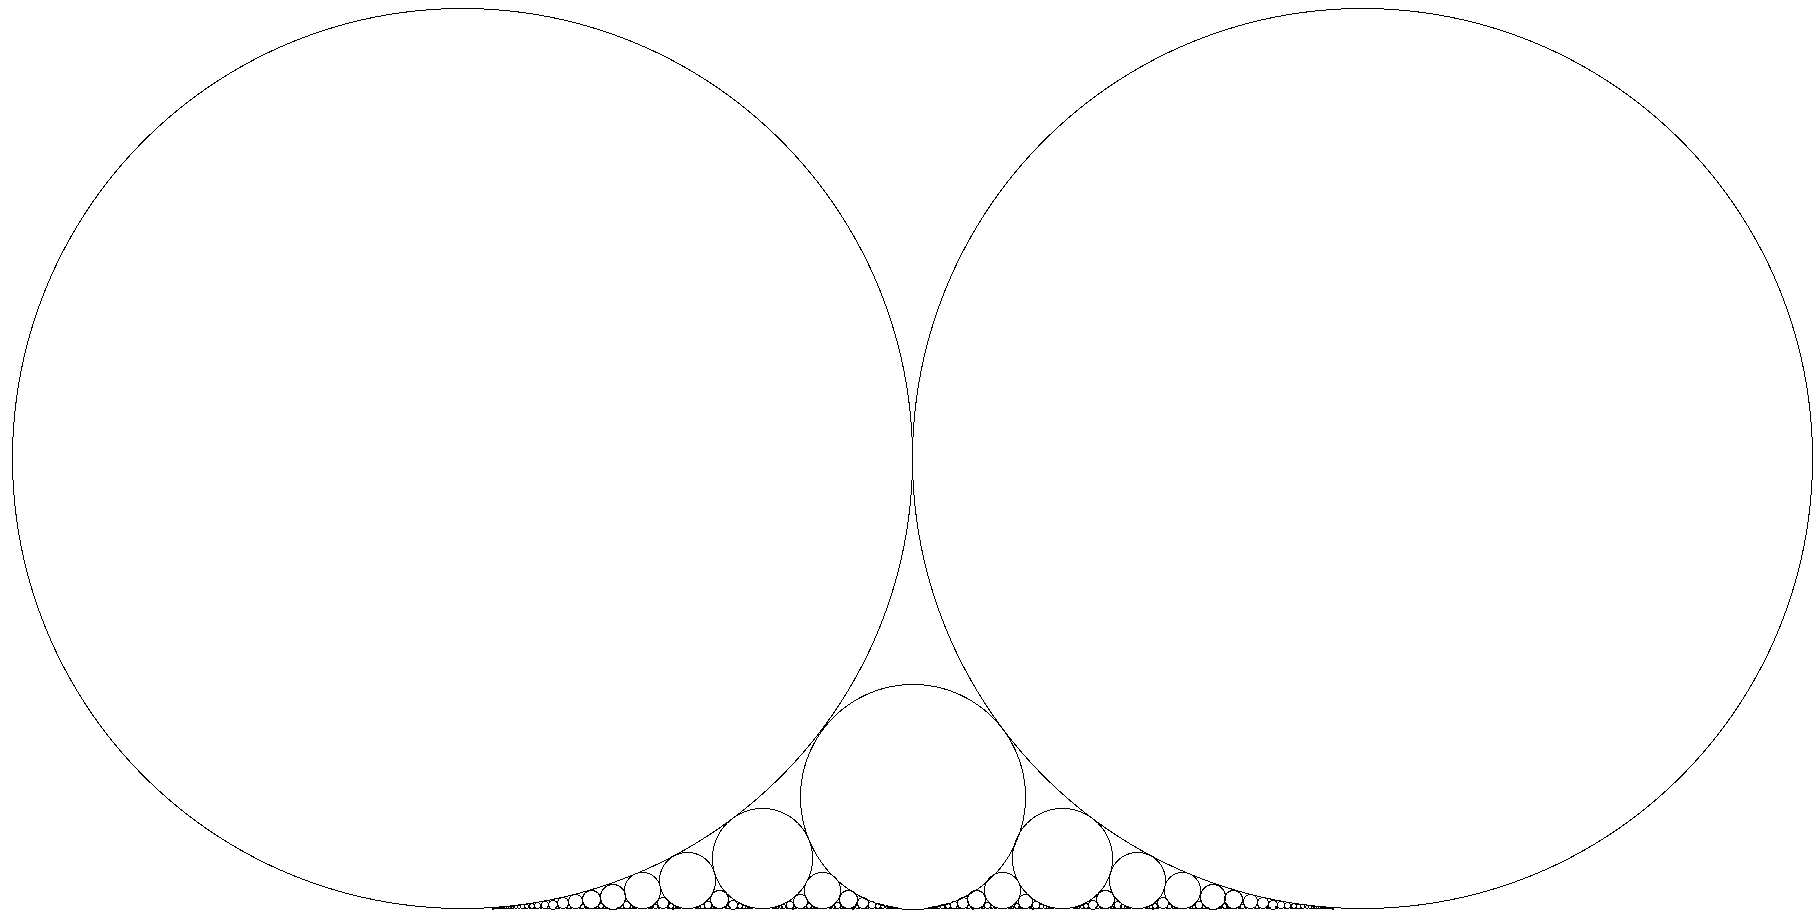
\includegraphics[width = \linewidth]{Sierpiński Arrowhead Curve/8.png}
		\caption{Iterate 8}
	\end{subfigure}
	\begin{subfigure}{0.18\linewidth}
		\includegraphics[width = \linewidth]{Sierpiński Arrowhead Curve/10.png}
		\caption{Iterate 10}
	\end{subfigure}
	\caption{Sierpi\'nski Arrowhead Curve for even iterates (why only even?)}
\end{figure}
\begin{funvideo}
	\href{https://youtu.be/UBuPWdSbyf8}{Unfolding The Dragon | Fractal Curve -- Think Twice}\\
	\href{https://youtu.be/gB9n2gHsHN4}{Fractals are typically not self-similar -- 3Blue1Brown}
\end{funvideo}
\subsection{Chaos Game (Iterated Function Systems)}
Intuitively, in these systems, we iterate a specific function repeatedly. For simplicity, let us only consider affine transformations\footnote{In general, affine transformations are of the form $Ax+b$ where $A$ is a matrix and $x,b$ are vectors.}. We take a random initial point $P=\begin{bmatrix}x\\y\end{bmatrix}$ and repeatedly apply different affine transformations to get $P_{\text{next}}=f_i(P)$ with some probability $p_i$. After large number of iterations, a pattern emerges!
\begin{equation}
	f(x,y)={\begin{bmatrix}a&b\\c&d\end{bmatrix}}{\begin{bmatrix}x\\y\end{bmatrix}}+{\begin{bmatrix}e\\f\end{bmatrix}}
\end{equation}
\begin{note}
	You can get probabilities by smartly generating random numbers. \verb!randuv(x, y)! (Simplecpp library) generates random numbers (\verb!double!) between $x$ and $y$. If you feel adventurous then implement your own randon number generator using \hyperref[pp:linearfeedbackshiftregister]{LFSRs} :).
\end{note}
% \vspace{-2em}
\subsubsection{Sierpi\'nski Triangle}{\label{pp:sierpinskitriangle}}
Consider $A,B,C$ as some co-ordinates of an equilateral triangle. Now, after taking a random initial point $P$ we go half the distance towards $A$ or $B$ or $C$ with equal probability and repeat this with the new point over and over. This operation can be representated using affine transformations as below
\begin{align}
	\text{With probability 1/3, apply }& \quad f_{1}(x,y) = {\begin{bmatrix}0.05&0.00\\0.00&0.05\end{bmatrix}}{\begin{bmatrix}x\\y\end{bmatrix}}+\frac{1}{2}{\begin{bmatrix}A_x \\ A_y \end{bmatrix}}\\
	\text{With probability 1/3, apply }& \quad f_{2}(x,y) = {\begin{bmatrix}0.05&0.00\\0.00&0.05\end{bmatrix}}{\begin{bmatrix}x\\y\end{bmatrix}}+\frac{1}{2}{\begin{bmatrix}B_x \\ B_y \end{bmatrix}}\\
	\text{With probability 1/3, apply }& \quad f_{3}(x,y) = {\begin{bmatrix}0.05&0.00\\0.00&0.05\end{bmatrix}}{\begin{bmatrix}x\\y\end{bmatrix}}+\frac{1}{2}{\begin{bmatrix}C_x \\ C_y \end{bmatrix}}
\end{align}
In limit, we get the Sierpi\'nski Triangle.

\textbf{Problem Statement:}\\
Simulate this system and observe the generated pattern using \verb!turtleSim! with appropriate scaling such that it takes same width and height for all iterates.
\begin{tcolorbox}[breakable, enhanced, sharpish corners]%, colback = white]
	\href{https://github.com/paramrathour/CS-101/tree/main/Starter Codes/Sierpiński Triangle.cpp}{\textbf{Starter Code}}
\end{tcolorbox}
\begin{figure}[H]
	\centering
	\begin{subfigure}{0.18\linewidth}
		\includegraphics[width = \linewidth]{Sierpiński Triangle/10.png}
		\caption{Iterate 10}
	\end{subfigure}
	\begin{subfigure}{0.18\linewidth}
		\includegraphics[width = \linewidth]{Sierpiński Triangle/100.png}
		\caption{Iterate 100}
	\end{subfigure}
	\begin{subfigure}{0.18\linewidth}
		\includegraphics[width = \linewidth]{Sierpiński Triangle/1000.png}
		\caption{Iterate 1000}
	\end{subfigure}
	\begin{subfigure}{0.18\linewidth}
		\includegraphics[width = \linewidth]{Sierpiński Triangle/10000.png}
		\caption{Iterate 10000}
	\end{subfigure}
	\begin{subfigure}{0.18\linewidth}
		\includegraphics[width = \linewidth]{Sierpiński Triangle/100000.png}
		\caption{Iterate 100000}
	\end{subfigure}
	\caption{Sierpi\'nski Triangle for iterates growing with power of 10}
\end{figure}
\vspace{-2em}
\subsubsection{Barnsley's Fern}{\label{pp:barnsleyfern}}
Again, by taking different $f_i$, we get different fractal. An explain
\begin{align}
	\text{With probability 0.01, apply }& \quad f_{1}(x,y) = {\begin{bmatrix}0.00&0.00\\0.00&0.16\end{bmatrix}}{\begin{bmatrix}x\\y\end{bmatrix}}\\
	\text{With probability 0.85, apply }& \quad f_{2}(x,y) = {\begin{bmatrix}0.85&0.04\\-0.04&0.85\end{bmatrix}}{\begin{bmatrix}x\\y\end{bmatrix}}+{\begin{bmatrix}0.00\\1.60\end{bmatrix}}\\
	\text{With probability 0.07, apply }& \quad f_{3}(x,y) = {\begin{bmatrix}0.20&-0.26\\0.23&0.22\end{bmatrix}}{\begin{bmatrix}x\\y\end{bmatrix}}+{\begin{bmatrix}0.00\\1.60\end{bmatrix}}\\
	\text{With probability 0.07, apply }& \quad f_{4}(x,y) = {\begin{bmatrix}-0.15&0.28\\0.26&0.24\end{bmatrix}}{\begin{bmatrix}x\\y\end{bmatrix}}+{\begin{bmatrix}0.00\\0.44\end{bmatrix}}
\end{align}
In limit, we get the Barnsley's Fern.

\textbf{Problem Statement:}\\
Simulate this system and observe the generated pattern using \verb!turtleSim! with appropriate scaling such that it takes same width and height for all iterates.
\begin{tcolorbox}[breakable, enhanced, sharpish corners]%, colback = white]
	\href{https://github.com/paramrathour/CS-101/tree/main/Starter Codes/Barnsley's Fern.cpp}{\textbf{Starter Code}}
\end{tcolorbox}
\begin{figure}[H]
	\centering
	\begin{subfigure}{0.22\linewidth}
		\includegraphics[width = \linewidth]{Barnsley's Fern/100.png}
		\caption{Iterate 100}
	\end{subfigure}
	\begin{subfigure}{0.22\linewidth}
		\includegraphics[width = \linewidth]{Barnsley's Fern/1000.png}
		\caption{Iterate 1000}
	\end{subfigure}
	\begin{subfigure}{0.22\linewidth}
		\includegraphics[width = \linewidth]{Barnsley's Fern/10000.png}
		\caption{Iterate 10000}
	\end{subfigure}
	\begin{subfigure}{0.22\linewidth}
		\includegraphics[width = \linewidth]{Barnsley's Fern/100000.png}
		\caption{Iterate 100000}
	\end{subfigure}
	\caption{Barnsley's Fern for iterates growing with power of 10}
\end{figure}
\begin{funvideo}
	\href{https://youtu.be/kbKtFN71Lfs}{Chaos Game -- Numberphile}\\
	\href{https://youtu.be/IGlGvSXkRGI}{Chaos Game | Fractals emerging from chaos | Computer simulation -- Think Twice}
\end{funvideo}